% --------------------------------------------------------------
% This is all preamble stuff that you don't have to worry about.
% Head down to where it says "Start here"
% --------------------------------------------------------------
 
\documentclass[12pt]{article}
 
\usepackage[margin=1in]{geometry} 
\usepackage{amsmath,amsthm,amssymb,scrextend}
\usepackage{fancyhdr}
\usepackage{enumitem}
\usepackage{amsmath}
\usepackage{amssymb}
\usepackage{textcomp}
\usepackage{fancybox}
\usepackage{tikz}
\usepackage{tasks}
\pagestyle{fancy}
\usepackage[makeroom]{cancel}
\usepackage{graphicx}
\usepackage{caption}
\usepackage{mwe}


\usepackage{tikz}
\usetikzlibrary{positioning}

\newenvironment{rcases}
  {\left.\begin{aligned}}
{\end{aligned}\right\rbrace}

\newcommand{\N}{\mathbb{N}}
\newcommand{\Z}{\mathbb{Z}}
\newcommand{\I}{\mathbb{I}}
\newcommand{\R}{\mathbb{R}}
\newcommand{\Q}{\mathbb{Q}}
\renewcommand{\qed}{\hfill$\blacksquare$}
\let\newproof\proof
\renewenvironment{proof}{\begin{addmargin}[1em]{0em}\begin{newproof}}{\end{newproof}\end{addmargin}\qed}
% \newcommand{\expl}[1]{\text{\hfill[#1]}$}
 
\newenvironment{theorem}[2][Theorem]{\begin{trivlist}
\item[\hskip \labelsep {\bfseries #1}\hskip \labelsep {\bfseries #2.}]}{\end{trivlist}}
\newenvironment{lemma}[2][Lemma]{\begin{trivlist}
\item[\hskip \labelsep {\bfseries #1}\hskip \labelsep {\bfseries #2.}]}{\end{trivlist}}
\newenvironment{problem}[2][Problem]{\begin{trivlist}
\item[\hskip \labelsep {\bfseries #1}\hskip \labelsep {\bfseries #2.}]}{\end{trivlist}}
\newenvironment{exercise}[2][Exercise]{\begin{trivlist}
\item[\hskip \labelsep {\bfseries #1}\hskip \labelsep {\bfseries #2.}]}{\end{trivlist}}
\newenvironment{reflection}[2][Reflection]{\begin{trivlist}
\item[\hskip \labelsep {\bfseries #1}\hskip \labelsep {\bfseries #2.}]}{\end{trivlist}}
\newenvironment{proposition}[2][Proposition]{\begin{trivlist}
\item[\hskip \labelsep {\bfseries #1}\hskip \labelsep {\bfseries #2.}]}{\end{trivlist}}
\newenvironment{corollary}[2][Corollary]{\begin{trivlist}
\item[\hskip \labelsep {\bfseries #1}\hskip \labelsep {\bfseries #2.}]}{\end{trivlist}}




\setlength{\parindent}{0pt}
\begin{document}
\setcounter{section}{3}

 \settasks{
	counter-format=(tsk[r]),
	label-width=4ex
}
% --------------------------------------------------------------
%                         Start here
% --------------------------------------------------------------

\lhead{Math 475}
\chead{Chapter 3}
\rhead{Meenmo K.}
\subsection{Pigeonhole Principle}
Given $n+1$ pigeons that we place into $n$ pigeonholes, then there 15 at least 1 pigeonhole containing 2 or more pigeons (Theorem 3.1.1).\\

{\bf Example} 
\begin{enumerate}
    \item Given 367 people, at least 2 share a birthday, suppose
    \begin{itemize}
        \item pigeon: people
        \item pigeonholes: 366 dates on the calendar
    \end{itemize}
    
    \item $n$ married couples ($2n$ people total). How many people must be selected to guarantee selection of a married couple? $n+1$\\
    
    \underline{Why?} Use pigeonhole principle.
    \begin{itemize}
        \item Pigeons: people ($2n$)
        \item Pigeonholes: each marriage as a category ($n$).\\
        By P.P., need $n+1$ for a repeat (2 people in same marriage).
    \end{itemize}
    
    \item Given $m$ integers $a_1,a_2,...,a_n,$ there exist integers $k$ and $l$ with $0\le k< l \le m$ such that $a_{k+1}+a_{k+2}+\ldots+a_l$ is divisible by $m$.
    \begin{itemize}
        \item pigeonholes: remainders upon division by $m$ ($m$ possibilities are 0,1,...,m-1).
        \item pigeons: we will start by considering the sums\\
        \begin{align}
            &a_1\nonumber \\
            &a_1+a_2+a_3\nonumber \\
            \vdots \nonumber \\
            &a_1+a_2+a_3+\ldots +a_m \nonumber
        \end{align}
    \end{itemize}
    
    \begin{itemize}
    \item[\sl Case 1:] Each of the $m$ pigeons fits into a different pigeonhole has 1 pigeon. So "remainder 0 pigeonhole" applies to one of these sums. So, there is a sum $a_1+a_2+a_3+\ldots +a_l$  divisible by $m$ and we are done.\\
    
    In fact, this happens any time one of these sums is divisible by $m$. \\
    
    \item[\sl Case 2:] No sum amongst our in $m$ sums is divisible by $m$. We now have $m-1$ pigeonholes and $m$ pigeons. By P.P., there exist $k$ and $l (l>k)$ such that $a_1+a_2+a_3+\ldots +a_k$ and $a_1+a_2+a_3+\ldots +a_{k+1}+\ldots +a_l$. Both have remainder $r$ when divided by $m$. So, $(a_1+a_2+a_3+\ldots +a_l)-(a_1+a_2+a_3+\ldots +a_k) = a_{k+1}+a_{k+2}+...+a_l$ is divisible by $m$. 
    \end{itemize}
    
    \item Chess master has 11 weeks to prepare. The master plays at least one game a day. But no more than 12 games during any calendar week. \\
    
    \underline{Goal: } Show there is some succession of consecutive days in which exactly 21 gives are played.\\
    
    Let $a_i$ be the total number of games played from day 1 through day 2. 
    $$1\le a_1<a_2<a_3<\ldots<a_{77}\le 132$$
    $$22\lea_1+21<a_2+21<\ldots<a_{77}+21\le 153$$
    
    \begin{itemize}
        \item pigeons: integers $a_1,a_2,...,a_{77},a_1+21,a_2+21,...,a_{77}+21$
        \item Pigeonholes: integers 1,2,...,153
    \end{itemize}
    
    By P.P., there are two of those integers that are equal.\\
    
    So, there exist $i$ and $j$ (where $i\neq j$) such that
    $$\underbrace{\xcancel{a_i=a_j}\text{ or }\xcancel{a_i+21=a_j+21}}_{\substack{\text{Impossible because at least}\\ \text{one game played per day}}}\text{ or }a_i=a_j+21$$
    
    So,$$a_i=a_j+21\Leftrightarrow \underbrace{a_i-a_j}_{\substack{\text{\# of games played from}\\ \text{day $j+1$ through day $i$}}}=21$$\\
    
    
    \item We choose 101 integers from 1,2,...,200. Show there are 2 such that 1 divides another.
    \begin{itemize}
        \item pigeons: 101 integers
        \item pigeonholes: Greatest odd factors of our integers.\\
        
        i.e., given $1\le n\le 200$, write $n=2^k\cdot a$ where a is odd.\\
        
        100 pigeonholes: a=1,3,5,7,9,...,199
        
        
    \end{itemize}
\end{enumerate}


\newpage
\subsection{Strong Form of Pigeonhole Principal}
{\bf Theorem 3.2.1} If $q_1\;q_2,\;\ldots,q_n$ are positive integers and $q_1+q_2+\ldots+q_n-n+1$ objects are placed into $n$ boxes then 
\begin{itemize}
    \item Box 1 has at least $q_1$ objects or
    \item Box 2 has at least $q_2$ objects or\\
    \vdots
    \item Box $n$ has at least $q_n$ objects
\end{itemize}

Previously, we considered $q_1=q_2=\ldots=q_n=2.$\\

{\bf Corollary 3.2.2} Let $n$ and $r$ be positive integers if $n(r-1)+1$ objects are distributed into $n$ boxes then there is at least one box containing at least $r$ objects.\\

This is {\sl Theorem 3.2.1} with $q_=q_2=\ldots =q_n=r$.\\

{\bf Example} Need a basket with at
\begin{itemize}
    \item at least 8 apples or 
    \item at least 6 bananas or 
    \item at least 9 oranges.
\end{itemize}

How many individual pieces of fruit do we need to achieve this?\\

$\Rightarrow$ By Theorem 3.2.1, we need 7+5+8+1=21 pieces of fruit.

\newpage
\subsection{Ramsey Numbers}
{\sl Goal: } Show that amongst any group of 6 people, there 3 people that either all know each other or all don't know each other. \\

{\sl Idea: } We will model this by considering colorings of the edges of a \underline{complete graph}.\\

A complete graph on $n$ vertices (called $K_n$) is a collection of $n$ vertices with one edge drawn between any given pair of vertices.
\begin{center}
    


\tikzset{every picture/.style={line width=0.75pt}} %set default line width to 0.75pt        

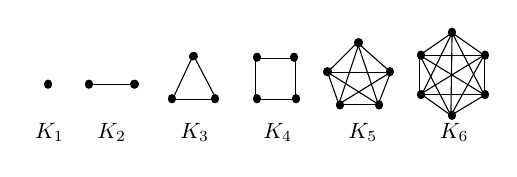
\begin{tikzpicture}[x=0.75pt,y=0.75pt,yscale=-1,xscale=1]
%uncomment if require: \path (0,541.6666564941406); %set diagram left start at 0, and has height of 541.6666564941406

%Shape: Free Drawing [id:dp7706007867329825] 
\draw  [color={rgb, 255:red, 0; green, 0; blue, 0 }  ][line width=3] [line join = round][line cap = round] (49.93,59.54) .. controls (49.93,59.69) and (49.93,59.84) .. (49.93,59.99) ;
%Shape: Free Drawing [id:dp1230610229805944] 
\draw  [color={rgb, 255:red, 0; green, 0; blue, 0 }  ][line width=3] [line join = round][line cap = round] (71.93,59.54) .. controls (71.93,59.69) and (71.93,59.84) .. (71.93,59.99) ;
%Shape: Free Drawing [id:dp8433888058688421] 
\draw  [color={rgb, 255:red, 0; green, 0; blue, 0 }  ][line width=3] [line join = round][line cap = round] (30.43,59.54) .. controls (30.43,59.69) and (30.43,59.84) .. (30.43,59.99) ;
%Straight Lines [id:da11718982707561376] 
\draw    (50,60) -- (72.43,60) ;


%Shape: Free Drawing [id:dp20394431608502583] 
\draw  [color={rgb, 255:red, 0; green, 0; blue, 0 }  ][line width=3] [line join = round][line cap = round] (89.93,66.54) .. controls (89.93,66.69) and (89.93,66.84) .. (89.93,66.99) ;
%Shape: Free Drawing [id:dp8917302290353502] 
\draw  [color={rgb, 255:red, 0; green, 0; blue, 0 }  ][line width=3] [line join = round][line cap = round] (110.93,66.54) .. controls (110.93,66.69) and (110.93,66.84) .. (110.93,66.99) ;
%Straight Lines [id:da28744692817355344] 
\draw    (89,67) -- (111.43,67) ;


%Shape: Free Drawing [id:dp04954593819278075] 
\draw  [color={rgb, 255:red, 0; green, 0; blue, 0 }  ][line width=3] [line join = round][line cap = round] (100.19,46.38) .. controls (100.32,46.3) and (100.45,46.22) .. (100.58,46.15) ;
%Straight Lines [id:da07263026981975895] 
\draw    (111.43,67) -- (100.34,45.71) ;


%Straight Lines [id:da15025084615430284] 
\draw    (89.92,67.87) -- (100.34,45.71) ;


%Shape: Rectangle [id:dp37406222940455813] 
\draw   (130.43,47.27) -- (149.43,47.27) -- (149.43,67) -- (130.43,67) -- cycle ;
%Shape: Free Drawing [id:dp17692584323059113] 
\draw  [color={rgb, 255:red, 0; green, 0; blue, 0 }  ][line width=3] [line join = round][line cap = round] (130.93,66.54) .. controls (130.93,66.69) and (130.93,66.84) .. (130.93,66.99) ;
%Shape: Free Drawing [id:dp7445652635386102] 
\draw  [color={rgb, 255:red, 0; green, 0; blue, 0 }  ][line width=3] [line join = round][line cap = round] (149.93,66.54) .. controls (149.93,66.69) and (149.93,66.84) .. (149.93,66.99) ;
%Shape: Free Drawing [id:dp7919819521300071] 
\draw  [color={rgb, 255:red, 0; green, 0; blue, 0 }  ][line width=3] [line join = round][line cap = round] (130.93,46.54) .. controls (130.93,46.69) and (130.93,46.84) .. (130.93,46.99) ;
%Shape: Free Drawing [id:dp9770363333251488] 
\draw  [color={rgb, 255:red, 0; green, 0; blue, 0 }  ][line width=3] [line join = round][line cap = round] (148.93,46.54) .. controls (148.93,46.69) and (148.93,46.84) .. (148.93,46.99) ;
%Shape: Free Drawing [id:dp8470669570889577] 
\draw  [color={rgb, 255:red, 0; green, 0; blue, 0 }  ][line width=3] [line join = round][line cap = round] (164.93,53.54) .. controls (164.93,53.69) and (164.93,53.84) .. (164.93,53.99) ;
%Shape: Free Drawing [id:dp06856864459772183] 
\draw  [color={rgb, 255:red, 0; green, 0; blue, 0 }  ][line width=3] [line join = round][line cap = round] (194.93,53.54) .. controls (194.93,53.69) and (194.93,53.84) .. (194.93,53.99) ;
%Shape: Free Drawing [id:dp20020706285555678] 
\draw  [color={rgb, 255:red, 0; green, 0; blue, 0 }  ][line width=3] [line join = round][line cap = round] (170.93,69.54) .. controls (170.93,69.69) and (170.93,69.84) .. (170.93,69.99) ;
%Shape: Free Drawing [id:dp9414367282654994] 
\draw  [color={rgb, 255:red, 0; green, 0; blue, 0 }  ][line width=3] [line join = round][line cap = round] (189.93,69.54) .. controls (189.93,69.69) and (189.93,69.84) .. (189.93,69.99) ;
%Shape: Free Drawing [id:dp38045620578549366] 
\draw  [color={rgb, 255:red, 0; green, 0; blue, 0 }  ][line width=3] [line join = round][line cap = round] (179.93,39.54) .. controls (179.93,39.69) and (179.93,39.84) .. (179.93,39.99) ;
%Straight Lines [id:da5718679671220828] 
\draw    (165,54) -- (189.43,69.4) ;


%Straight Lines [id:da9766699703205965] 
\draw    (169.43,69.4) -- (189.43,69.4) ;


%Straight Lines [id:da025336785157494157] 
\draw    (189.43,69.4) -- (179.34,39.71) ;


%Straight Lines [id:da08837520252141506] 
\draw    (165,54) -- (195.43,54) ;


%Straight Lines [id:da7623297516045588] 
\draw    (170.43,69.4) -- (180.34,39.71) ;


%Straight Lines [id:da5948102558666608] 
\draw    (165,54) -- (179.34,39.71) ;


%Straight Lines [id:da24401432990133376] 
\draw    (195.43,54) -- (179.34,39.71) ;


%Straight Lines [id:da43365053941250875] 
\draw    (170.43,69.4) -- (165,54) ;


%Straight Lines [id:da0658788800960759] 
\draw    (189.43,69.4) -- (195.43,54) ;


%Straight Lines [id:da22845168721642417] 
\draw    (195.43,54) -- (170.43,69.4) ;


%Shape: Free Drawing [id:dp9814694734984799] 
\draw  [color={rgb, 255:red, 0; green, 0; blue, 0 }  ][line width=3] [line join = round][line cap = round] (209.93,64.54) .. controls (209.93,64.69) and (209.93,64.84) .. (209.93,64.99) ;
%Shape: Free Drawing [id:dp5404102323451001] 
\draw  [color={rgb, 255:red, 0; green, 0; blue, 0 }  ][line width=3] [line join = round][line cap = round] (240.93,64.54) .. controls (240.93,64.69) and (240.93,64.84) .. (240.93,64.99) ;
%Shape: Free Drawing [id:dp4162438898080709] 
\draw  [color={rgb, 255:red, 0; green, 0; blue, 0 }  ][line width=3] [line join = round][line cap = round] (209.93,45.54) .. controls (209.93,45.69) and (209.93,45.84) .. (209.93,45.99) ;
%Shape: Free Drawing [id:dp2274630842019849] 
\draw  [color={rgb, 255:red, 0; green, 0; blue, 0 }  ][line width=3] [line join = round][line cap = round] (240.93,45.54) .. controls (240.93,45.69) and (240.93,45.84) .. (240.93,45.99) ;
%Shape: Free Drawing [id:dp9108538552756342] 
\draw  [color={rgb, 255:red, 0; green, 0; blue, 0 }  ][line width=3] [line join = round][line cap = round] (224.93,74.54) .. controls (224.93,74.69) and (224.93,74.84) .. (224.93,74.99) ;
%Shape: Free Drawing [id:dp3708525162657317] 
\draw  [color={rgb, 255:red, 0; green, 0; blue, 0 }  ][line width=3] [line join = round][line cap = round] (224.93,34.54) .. controls (224.93,34.69) and (224.93,34.84) .. (224.93,34.99) ;
%Straight Lines [id:da7530430930074483] 
\draw    (225,35) -- (240.43,45.8) ;


%Straight Lines [id:da038430093946626] 
\draw    (225,35) -- (209.43,45.8) ;


%Straight Lines [id:da6946964643782292] 
\draw    (224.43,74.8) -- (210.43,64.8) ;


%Straight Lines [id:da8800539431610181] 
\draw    (239.43,65.8) -- (224.43,74.8) ;


%Straight Lines [id:da6969227487642842] 
\draw    (209.43,64.8) -- (209.43,45.8) ;


%Straight Lines [id:da6845536131435246] 
\draw    (240.43,64.8) -- (240.43,45.8) ;


%Straight Lines [id:da3115502111339148] 
\draw    (209.43,45.8) -- (239.87,45.8) ;


%Straight Lines [id:da6469427256721771] 
\draw    (210.43,64.8) -- (240.87,64.8) ;


%Straight Lines [id:da9977281688285915] 
\draw    (224.43,74.8) -- (225,35) ;


%Straight Lines [id:da20771908338188338] 
\draw    (240.43,64.8) -- (209.43,45.8) ;


%Straight Lines [id:da10305048079548706] 
\draw    (240.43,45.8) -- (209.43,64.8) ;


%Straight Lines [id:da46191637040154143] 
\draw    (224.43,74.8) -- (209.43,45.8) ;


%Straight Lines [id:da12883904861734408] 
\draw    (224.43,74.8) -- (240.43,45.8) ;


%Straight Lines [id:da8733798157320598] 
\draw    (210.43,64.8) -- (225,35) ;


%Straight Lines [id:da8418728512222313] 
\draw    (240.43,64.8) -- (225,35) ;



% Text Node
\draw (31,83) node [scale=0.8] [align=left] {$K_1$};
% Text Node
\draw (61,83) node [scale=0.8] [align=left] {$K_2$};
% Text Node
\draw (101,83) node [scale=0.8] [align=left] {$K_3$};
% Text Node
\draw (141,83) node [scale=0.8] [align=left] {$K_4$};
% Text Node
\draw (182,83) node [scale=0.8] [align=left] {$K_5$};
% Text Node
\draw (226,83) node [scale=0.8] [align=left] {$K_6$};


\end{tikzpicture}

\end{center}
We represent 6 people as vertices of a $K_6$ and we draw a red edge between them if they know each other.\\

So, our goal boils down to showing that, if we color the edges of $K_6$ either red or blue, we obtain either a red $K_3$ or a blue $K_3$ within our $K_6$.

\begin{center}
\tikzset{every picture/.style={line width=0.75pt}} %set default line width to 0.75pt        

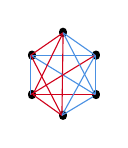
\begin{tikzpicture}[x=0.75pt,y=0.75pt,yscale=-1,xscale=1]
%uncomment if require: \path (0,541.6666564941406); %set diagram left start at 0, and has height of 541.6666564941406

%Shape: Free Drawing [id:dp39586824535787013] 
\draw  [color={rgb, 255:red, 0; green, 0; blue, 0 }  ][line width=3] [line join = round][line cap = round] (18.93,31.54) .. controls (18.93,31.69) and (18.93,31.84) .. (18.93,31.99) ;
%Shape: Free Drawing [id:dp897297811559653] 
\draw  [color={rgb, 255:red, 0; green, 0; blue, 0 }  ][line width=3] [line join = round][line cap = round] (49.93,31.54) .. controls (49.93,31.69) and (49.93,31.84) .. (49.93,31.99) ;
%Shape: Free Drawing [id:dp5168514273590323] 
\draw  [color={rgb, 255:red, 0; green, 0; blue, 0 }  ][line width=3] [line join = round][line cap = round] (18.93,12.54) .. controls (18.93,12.69) and (18.93,12.84) .. (18.93,12.99) ;
%Shape: Free Drawing [id:dp3921582724458679] 
\draw  [color={rgb, 255:red, 0; green, 0; blue, 0 }  ][line width=3] [line join = round][line cap = round] (49.93,12.54) .. controls (49.93,12.69) and (49.93,12.84) .. (49.93,12.99) ;
%Shape: Free Drawing [id:dp7766485395370373] 
\draw  [color={rgb, 255:red, 0; green, 0; blue, 0 }  ][line width=3] [line join = round][line cap = round] (33.93,41.54) .. controls (33.93,41.69) and (33.93,41.84) .. (33.93,41.99) ;
%Shape: Free Drawing [id:dp4290756952863908] 
\draw  [color={rgb, 255:red, 0; green, 0; blue, 0 }  ][line width=3] [line join = round][line cap = round] (33.93,1.54) .. controls (33.93,1.69) and (33.93,1.84) .. (33.93,1.99) ;
%Straight Lines [id:da8588835526498475] 
\draw [color={rgb, 255:red, 74; green, 144; blue, 226 }  ,draw opacity=1 ]   (34,2) -- (49.43,12.8) ;


%Straight Lines [id:da5210713387579642] 
\draw [color={rgb, 255:red, 208; green, 2; blue, 27 }  ,draw opacity=1 ]   (34,2) -- (18.43,12.8) ;


%Straight Lines [id:da4495272849148053] 
\draw [color={rgb, 255:red, 208; green, 2; blue, 27 }  ,draw opacity=1 ]   (33.43,41.8) -- (19.43,31.8) ;


%Straight Lines [id:da09404038562873573] 
\draw [color={rgb, 255:red, 74; green, 144; blue, 226 }  ,draw opacity=1 ]   (48.43,32.8) -- (33.43,41.8) ;


%Straight Lines [id:da8995277347284591] 
\draw [color={rgb, 255:red, 74; green, 144; blue, 226 }  ,draw opacity=1 ]   (18.43,31.8) -- (18.43,12.8) ;


%Straight Lines [id:da44436664114988944] 
\draw [color={rgb, 255:red, 74; green, 144; blue, 226 }  ,draw opacity=1 ]   (49.43,31.8) -- (49.43,12.8) ;


%Straight Lines [id:da7923162418010703] 
\draw [color={rgb, 255:red, 74; green, 144; blue, 226 }  ,draw opacity=1 ]   (18.43,12.8) -- (48.87,12.8) ;


%Straight Lines [id:da22847825354789886] 
\draw [color={rgb, 255:red, 208; green, 2; blue, 27 }  ,draw opacity=1 ]   (19.43,31.8) -- (49.87,31.8) ;


%Straight Lines [id:da7493424785718721] 
\draw [color={rgb, 255:red, 208; green, 2; blue, 27 }  ,draw opacity=1 ]   (33.43,41.8) -- (34,2) ;


%Straight Lines [id:da40460859343382527] 
\draw [color={rgb, 255:red, 74; green, 144; blue, 226 }  ,draw opacity=1 ]   (49.43,31.8) -- (18.43,12.8) ;


%Straight Lines [id:da21976612508750737] 
\draw [color={rgb, 255:red, 208; green, 2; blue, 27 }  ,draw opacity=1 ]   (49.43,12.8) -- (18.43,31.8) ;


%Straight Lines [id:da9521491136817894] 
\draw [color={rgb, 255:red, 208; green, 2; blue, 27 }  ,draw opacity=1 ]   (33.43,41.8) -- (18.43,12.8) ;


%Straight Lines [id:da458797543748404] 
\draw [color={rgb, 255:red, 74; green, 144; blue, 226 }  ,draw opacity=1 ]   (33.43,41.8) -- (49.43,12.8) ;


%Straight Lines [id:da35743425656124006] 
\draw [color={rgb, 255:red, 208; green, 2; blue, 27 }  ,draw opacity=1 ]   (19.43,31.8) -- (34,2) ;


%Straight Lines [id:da4906208903599707] 
\draw [color={rgb, 255:red, 74; green, 144; blue, 226 }  ,draw opacity=1 ]   (49.43,31.8) -- (34,2) ;

\end{tikzpicture}

\end{center}
Why does this happen?\\

Fix a vertex of our $K_6$. There are 5 edges connected to this vertex. By Pigeonhole Principal, at least 3 of these edges are red or blue. 
\begin{center}
    


\tikzset{every picture/.style={line width=0.75pt}} %set default line width to 0.75pt        

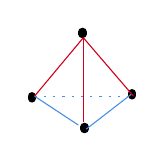
\begin{tikzpicture}[x=0.75pt,y=0.75pt,yscale=-1,xscale=1]
%uncomment if require: \path (0,541.6666564941406); %set diagram left start at 0, and has height of 541.6666564941406

%Straight Lines [id:da26761636911500397] 
\draw [color={rgb, 255:red, 74; green, 144; blue, 226 }  ,draw opacity=1 ] [dash pattern={on 0.84pt off 2.51pt}]  (226.72,209.02) -- (272.01,209.02) ;


%Shape: Free Drawing [id:dp9453750573042257] 
\draw  [color={rgb, 255:red, 0; green, 0; blue, 0 }  ][line width=3] [line join = round][line cap = round] (249.84,178.01) .. controls (249.84,178.36) and (249.84,178.72) .. (249.84,179.07) ;
%Shape: Free Drawing [id:dp8850338841104839] 
\draw  [color={rgb, 255:red, 0; green, 0; blue, 0 }  ][line width=3] [line join = round][line cap = round] (273.83,207.56) .. controls (273.83,207.91) and (273.83,208.27) .. (273.83,208.62) ;
%Shape: Free Drawing [id:dp7468929605021624] 
\draw  [color={rgb, 255:red, 0; green, 0; blue, 0 }  ][line width=3] [line join = round][line cap = round] (250.84,223.81) .. controls (250.84,224.16) and (250.84,224.52) .. (250.84,224.87) ;
%Shape: Free Drawing [id:dp9229039661926857] 
\draw  [color={rgb, 255:red, 0; green, 0; blue, 0 }  ][line width=3] [line join = round][line cap = round] (225.43,209.03) .. controls (225.43,209.39) and (225.43,209.74) .. (225.43,210.1) ;
%Straight Lines [id:da9656741938733711] 
\draw [color={rgb, 255:red, 74; green, 144; blue, 226 }  ,draw opacity=1 ]   (226.72,209.02) -- (247.82,222.91) ;


%Straight Lines [id:da05313018937734304] 
\draw [color={rgb, 255:red, 74; green, 144; blue, 226 }  ,draw opacity=1 ]   (251.66,224.87) -- (273.43,208.02) ;


%Straight Lines [id:da19977085518631532] 
\draw [color={rgb, 255:red, 208; green, 2; blue, 27 }  ,draw opacity=1 ]   (250.24,180.85) -- (250.24,221.43) ;


%Straight Lines [id:da9163617874588035] 
\draw [color={rgb, 255:red, 208; green, 2; blue, 27 }  ,draw opacity=1 ]   (250.24,180.85) -- (226.72,209.02) ;


%Straight Lines [id:da47631990709145167] 
\draw [color={rgb, 255:red, 208; green, 2; blue, 27 }  ,draw opacity=1 ]   (250.24,180.85) -- (274.43,209.02) ;


\end{tikzpicture}

\end{center}
If any of the vertices connecting these edges are connected by the same color edge, there is a $K_3$ of that color. If not, these edges for a $K_3$ of the other color. 

\vspace{2\baselineskip}
Feb 19, 2019(Tue)\\
Last time, we showed $K_6\rightarrow K_3,\;K_3$.\\

{\bf Theorem 3.3.1 Ramsey's Theorem} \\
If $m,n \ge 2$ are integers then there is a positive integer $p$ such that $$K_p\rightarrow K_m,K_n$$
i.e., given $m$ and $n$, then there is a $p$ such that 2-coloring the edges of $K_p$ gives a $K_m$ of one color \underline{or} a $K_n$ of another color.\\

Given $m$ and $n$ (integers $\ge 2$), there is a smallest value $p$ such that $K_p\rightarrow K_m,K_n$. We call this $p$ the Ramsey number of $m$ and $n$, notated $r(m,n)$.\\

\underline{Facts}
$$r(3,3)=6\qquad r(2,n)=n\qquad r(m,2)=m$$\\

{\sl Proof outline} We double induct on both $m$ and $n$.
\begin{itemize}
    \item[] Base Cases: $m=2$ and $n=2$\\ 
    Since $r(m,2)$ and $r(2,n)$ exist, the theorem is true for $m=2$ and $n=2$.\\
    
    \item[] Induction Hypothesis\\
    Assume $m\ge 3$ and $n\ge 3$. Assume $r(m,n-1)$ and $r(m-1,n)$ both exist. Let $p=r(m,n-1)+r(m-1,n)$. Suppose each edge of $K_p$ is colored either red or blue.
\end{itemize}

\vspace{1.5\baselineskip}
Let $x$ be a vertex of $K_p$.
\begin{center}
    


\tikzset{every picture/.style={line width=0.75pt}} %set default line width to 0.75pt        

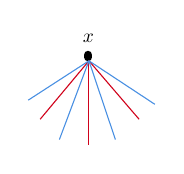
\begin{tikzpicture}[x=0.75pt,y=0.75pt,yscale=-1,xscale=1]
%uncomment if require: \path (0,541.6666564941406); %set diagram left start at 0, and has height of 541.6666564941406

%Shape: Free Drawing [id:dp901514751441314] 
\draw  [color={rgb, 255:red, 0; green, 0; blue, 0 }  ][line width=3] [line join = round][line cap = round] (363.84,34.01) .. controls (363.84,34.36) and (363.84,34.72) .. (363.84,35.07) ;
%Straight Lines [id:da20389982940952023] 
\draw [color={rgb, 255:red, 208; green, 2; blue, 27 }  ,draw opacity=1 ]   (364.24,36.85) -- (364.24,77.43) ;


%Straight Lines [id:da049941881654319786] 
\draw [color={rgb, 255:red, 208; green, 2; blue, 27 }  ,draw opacity=1 ]   (364.24,36.85) -- (340.72,65.02) ;


%Straight Lines [id:da4646535283130655] 
\draw [color={rgb, 255:red, 208; green, 2; blue, 27 }  ,draw opacity=1 ]   (364.24,36.85) -- (388.43,65.02) ;


%Straight Lines [id:da5051682903734711] 
\draw [color={rgb, 255:red, 74; green, 144; blue, 226 }  ,draw opacity=1 ]   (364.24,36.85) -- (350,74.8) ;


%Straight Lines [id:da30972162639678746] 
\draw [color={rgb, 255:red, 74; green, 144; blue, 226 }  ,draw opacity=1 ]   (364.24,36.85) -- (377,74.8) ;


%Straight Lines [id:da06970588851250104] 
\draw [color={rgb, 255:red, 74; green, 144; blue, 226 }  ,draw opacity=1 ]   (364.24,36.85) -- (396,57.8) ;


%Straight Lines [id:da6575220587658586] 
\draw [color={rgb, 255:red, 74; green, 144; blue, 226 }  ,draw opacity=1 ]   (364.24,36.85) -- (335,55.8) ;



% Text Node
\draw (364,26) node [scale=0.7] [align=left] {$x$};


\end{tikzpicture}
\end{center}
Let $R_x$ be the vertices connected to $x$ with a red edge and $B_x$ be the vertices connected to $x$ with a blue edge.
$$|R_x|+|B_x|=p-1=r(m,\;n-1)+r(m-1,\;n)-1$$
So, \begin{equation*}
\begin{rcases}
           |R_x| &\ge r(m-1,\;n) \\
\text{or } |B_x| &\ge r(m,\;n-1) 
\end{rcases}
\substack{\text{If both false then} \\ \text{$|R_x|+|B_x|\le p-2$}}
\end{equation*}

Either way, we have a red $K_m$ or a blue $K_n$.\\

This proof shows
\begin{align*}
    r(m,n) \le r(m-1,n)+r(m,n-1) \tag{m,n$\ge$ 3} 
\end{align*}

Let 
\begin{align*}
    f(m,\;n) &= \binom{m+n-2}{m-1} \tag{m,n$\ge$2}\\
    \binom{m+n-2}{m-1}&=\binom{m+n-3}{m-1}+\binom{m+n-3}{m-2} \tag{Pascal's Formula}
\end{align*}
So,
\begin{align*}
    f(m,n)&=f(m,n-1)+f(m-1,n)\\
    r(m,n)&\le\binom{m+n-2}{m-1}
\end{align*}

\end{document}